% Created by tikzDevice version 0.12.6 on 2025-04-07 20:34:28
% !TEX encoding = UTF-8 Unicode
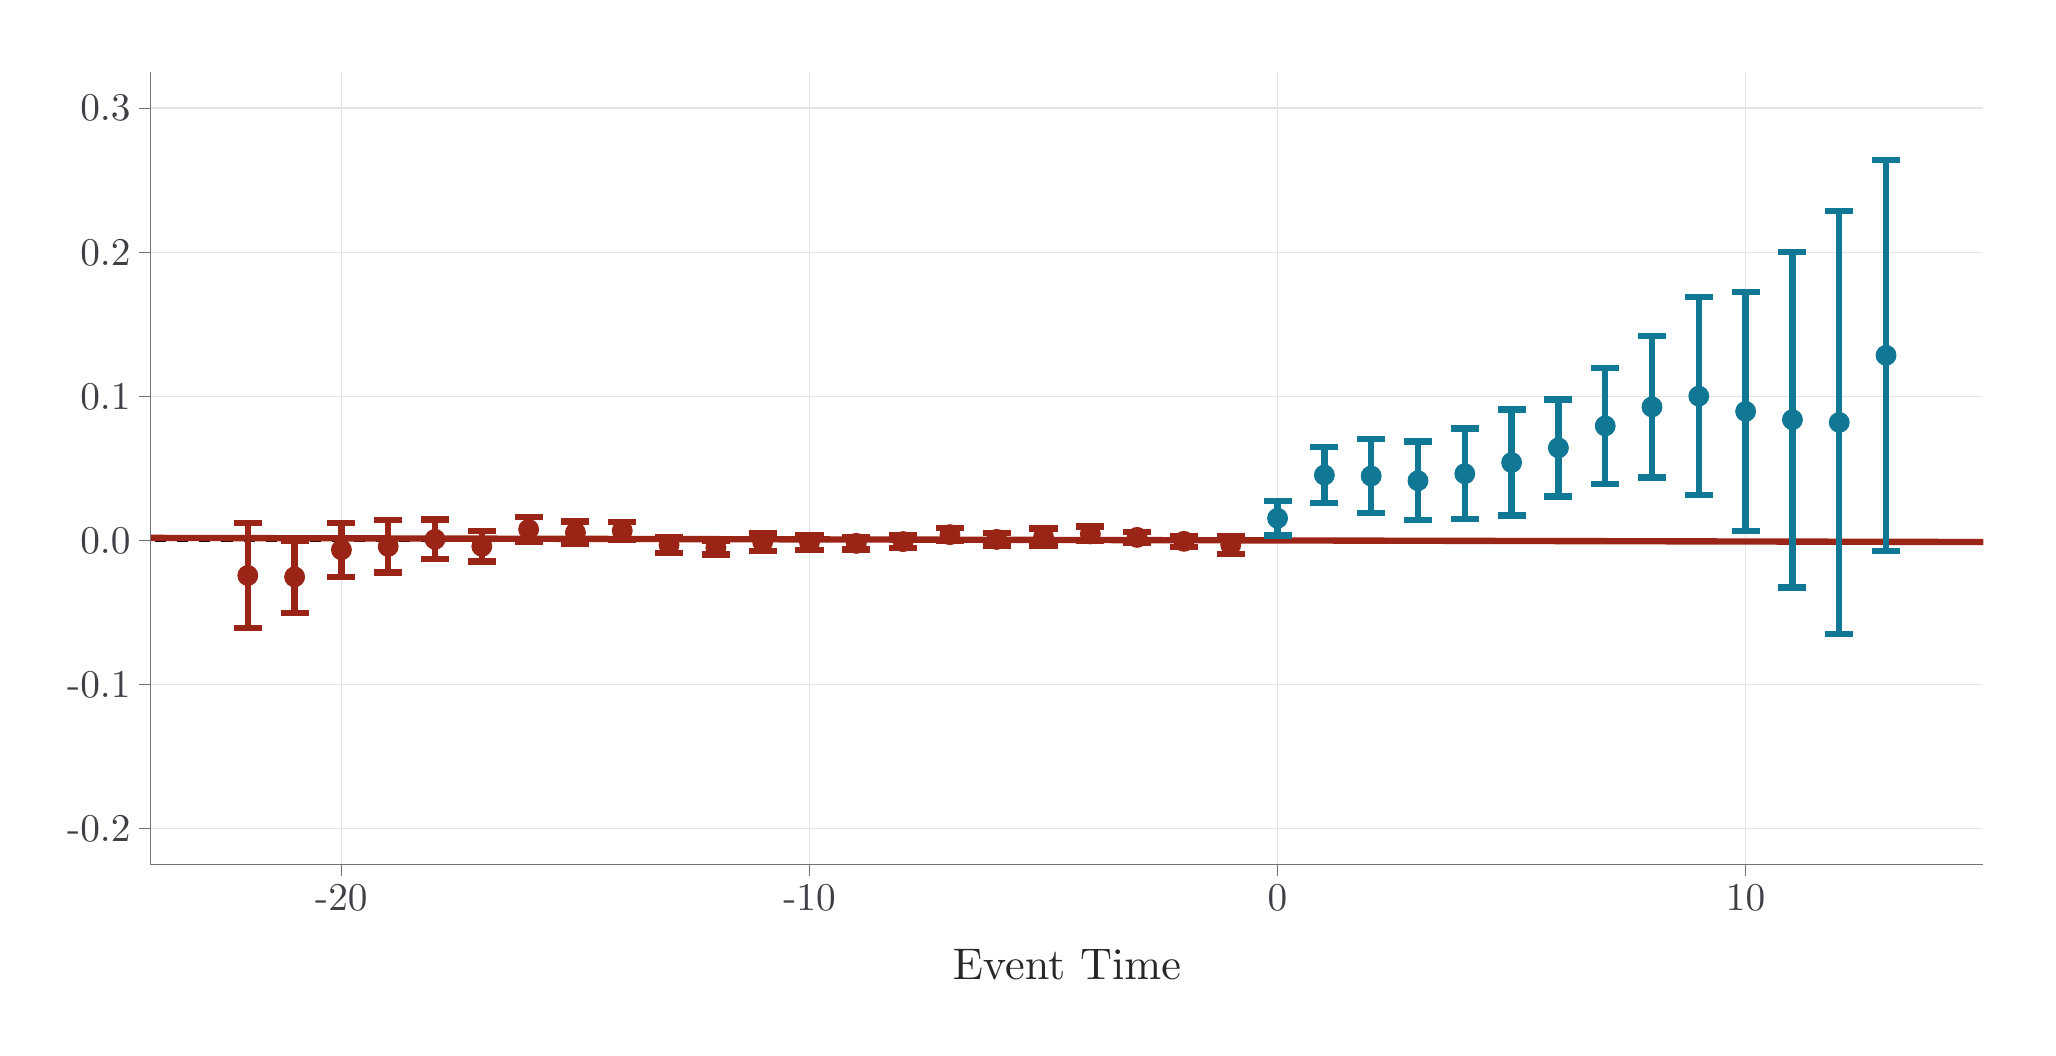
\begin{tikzpicture}[x=1pt,y=1pt]
\definecolor{fillColor}{RGB}{255,255,255}
\path[use as bounding box,fill=fillColor] (0,0) rectangle (722.70,361.35);
\begin{scope}
\path[clip] (  0.00,  0.00) rectangle (722.70,361.35);
\definecolor{drawColor}{RGB}{255,255,255}

\path[draw=drawColor,line width= 0.8pt,line join=round,line cap=round,fill=fillColor] (  0.00,  0.00) rectangle (722.70,361.35);
\end{scope}
\begin{scope}
\path[clip] ( 44.36, 58.90) rectangle (706.70,345.35);
\definecolor{drawColor}{RGB}{255,255,255}
\definecolor{fillColor}{RGB}{255,255,255}

\path[draw=drawColor,line width= 0.8pt,line join=round,line cap=round,fill=fillColor] ( 44.36, 58.90) rectangle (706.70,345.35);
\definecolor{drawColor}{RGB}{228,228,231}

\path[draw=drawColor,line width= 0.4pt,line join=round] ( 44.36, 71.92) --
	(706.70, 71.92);

\path[draw=drawColor,line width= 0.4pt,line join=round] ( 44.36,124.00) --
	(706.70,124.00);

\path[draw=drawColor,line width= 0.4pt,line join=round] ( 44.36,176.08) --
	(706.70,176.08);

\path[draw=drawColor,line width= 0.4pt,line join=round] ( 44.36,228.17) --
	(706.70,228.17);

\path[draw=drawColor,line width= 0.4pt,line join=round] ( 44.36,280.25) --
	(706.70,280.25);

\path[draw=drawColor,line width= 0.4pt,line join=round] ( 44.36,332.33) --
	(706.70,332.33);

\path[draw=drawColor,line width= 0.4pt,line join=round] (113.37, 58.90) --
	(113.37,345.35);

\path[draw=drawColor,line width= 0.4pt,line join=round] (282.50, 58.90) --
	(282.50,345.35);

\path[draw=drawColor,line width= 0.4pt,line join=round] (451.64, 58.90) --
	(451.64,345.35);

\path[draw=drawColor,line width= 0.4pt,line join=round] (620.78, 58.90) --
	(620.78,345.35);
\definecolor{drawColor}{RGB}{0,0,0}

\path[draw=drawColor,line width= 0.9pt,dash pattern=on 4pt off 4pt ,line join=round] (-617.98,176.08) -- (1369.04,176.08);
\definecolor{drawColor}{RGB}{154,36,21}

\path[draw=drawColor,line width= 2.3pt,line join=round] (-617.98,178.47) -- (1369.04,173.99);
\definecolor{fillColor}{RGB}{154,36,21}

\path[draw=drawColor,line width= 0.4pt,line join=round,line cap=round,fill=fillColor] ( 79.54,163.39) circle (  3.57);

\path[draw=drawColor,line width= 0.4pt,line join=round,line cap=round,fill=fillColor] ( 96.45,162.90) circle (  3.57);

\path[draw=drawColor,line width= 0.4pt,line join=round,line cap=round,fill=fillColor] (113.37,172.68) circle (  3.57);

\path[draw=drawColor,line width= 0.4pt,line join=round,line cap=round,fill=fillColor] (130.28,173.89) circle (  3.57);

\path[draw=drawColor,line width= 0.4pt,line join=round,line cap=round,fill=fillColor] (147.19,176.46) circle (  3.57);

\path[draw=drawColor,line width= 0.4pt,line join=round,line cap=round,fill=fillColor] (164.11,173.94) circle (  3.57);

\path[draw=drawColor,line width= 0.4pt,line join=round,line cap=round,fill=fillColor] (181.02,180.05) circle (  3.57);

\path[draw=drawColor,line width= 0.4pt,line join=round,line cap=round,fill=fillColor] (197.94,178.91) circle (  3.57);

\path[draw=drawColor,line width= 0.4pt,line join=round,line cap=round,fill=fillColor] (214.85,179.57) circle (  3.57);

\path[draw=drawColor,line width= 0.4pt,line join=round,line cap=round,fill=fillColor] (231.76,174.47) circle (  3.57);

\path[draw=drawColor,line width= 0.4pt,line join=round,line cap=round,fill=fillColor] (248.68,173.49) circle (  3.57);

\path[draw=drawColor,line width= 0.4pt,line join=round,line cap=round,fill=fillColor] (265.59,175.49) circle (  3.57);

\path[draw=drawColor,line width= 0.4pt,line join=round,line cap=round,fill=fillColor] (282.50,175.37) circle (  3.57);

\path[draw=drawColor,line width= 0.4pt,line join=round,line cap=round,fill=fillColor] (299.42,175.00) circle (  3.57);

\path[draw=drawColor,line width= 0.4pt,line join=round,line cap=round,fill=fillColor] (316.33,175.64) circle (  3.57);

\path[draw=drawColor,line width= 0.4pt,line join=round,line cap=round,fill=fillColor] (333.25,178.15) circle (  3.57);

\path[draw=drawColor,line width= 0.4pt,line join=round,line cap=round,fill=fillColor] (350.16,176.43) circle (  3.57);

\path[draw=drawColor,line width= 0.4pt,line join=round,line cap=round,fill=fillColor] (367.07,177.22) circle (  3.57);

\path[draw=drawColor,line width= 0.4pt,line join=round,line cap=round,fill=fillColor] (383.99,178.42) circle (  3.57);

\path[draw=drawColor,line width= 0.4pt,line join=round,line cap=round,fill=fillColor] (400.90,177.16) circle (  3.57);

\path[draw=drawColor,line width= 0.4pt,line join=round,line cap=round,fill=fillColor] (417.81,175.74) circle (  3.57);

\path[draw=drawColor,line width= 0.4pt,line join=round,line cap=round,fill=fillColor] (434.73,174.43) circle (  3.57);
\definecolor{drawColor}{RGB}{16,120,149}
\definecolor{fillColor}{RGB}{16,120,149}

\path[draw=drawColor,line width= 0.4pt,line join=round,line cap=round,fill=fillColor] (451.64,184.08) circle (  3.57);

\path[draw=drawColor,line width= 0.4pt,line join=round,line cap=round,fill=fillColor] (468.56,199.68) circle (  3.57);

\path[draw=drawColor,line width= 0.4pt,line join=round,line cap=round,fill=fillColor] (485.47,199.35) circle (  3.57);

\path[draw=drawColor,line width= 0.4pt,line join=round,line cap=round,fill=fillColor] (502.38,197.63) circle (  3.57);

\path[draw=drawColor,line width= 0.4pt,line join=round,line cap=round,fill=fillColor] (519.30,200.16) circle (  3.57);

\path[draw=drawColor,line width= 0.4pt,line join=round,line cap=round,fill=fillColor] (536.21,204.21) circle (  3.57);

\path[draw=drawColor,line width= 0.4pt,line join=round,line cap=round,fill=fillColor] (553.12,209.52) circle (  3.57);

\path[draw=drawColor,line width= 0.4pt,line join=round,line cap=round,fill=fillColor] (570.04,217.44) circle (  3.57);

\path[draw=drawColor,line width= 0.4pt,line join=round,line cap=round,fill=fillColor] (586.95,224.30) circle (  3.57);

\path[draw=drawColor,line width= 0.4pt,line join=round,line cap=round,fill=fillColor] (603.86,228.21) circle (  3.57);

\path[draw=drawColor,line width= 0.4pt,line join=round,line cap=round,fill=fillColor] (620.78,222.68) circle (  3.57);

\path[draw=drawColor,line width= 0.4pt,line join=round,line cap=round,fill=fillColor] (637.69,219.70) circle (  3.57);

\path[draw=drawColor,line width= 0.4pt,line join=round,line cap=round,fill=fillColor] (654.61,218.71) circle (  3.57);

\path[draw=drawColor,line width= 0.4pt,line join=round,line cap=round,fill=fillColor] (671.52,242.96) circle (  3.57);
\definecolor{drawColor}{RGB}{154,36,21}

\path[draw=drawColor,line width= 2.3pt,line join=round] ( 74.47,182.35) --
	( 84.61,182.35);

\path[draw=drawColor,line width= 2.3pt,line join=round] ( 79.54,182.35) --
	( 79.54,144.42);

\path[draw=drawColor,line width= 2.3pt,line join=round] ( 74.47,144.42) --
	( 84.61,144.42);

\path[draw=drawColor,line width= 2.3pt,line join=round] ( 91.38,175.89) --
	(101.53,175.89);

\path[draw=drawColor,line width= 2.3pt,line join=round] ( 96.45,175.89) --
	( 96.45,149.91);

\path[draw=drawColor,line width= 2.3pt,line join=round] ( 91.38,149.91) --
	(101.53,149.91);

\path[draw=drawColor,line width= 2.3pt,line join=round] (108.29,182.44) --
	(118.44,182.44);

\path[draw=drawColor,line width= 2.3pt,line join=round] (113.37,182.44) --
	(113.37,162.92);

\path[draw=drawColor,line width= 2.3pt,line join=round] (108.29,162.92) --
	(118.44,162.92);

\path[draw=drawColor,line width= 2.3pt,line join=round] (125.21,183.38) --
	(135.36,183.38);

\path[draw=drawColor,line width= 2.3pt,line join=round] (130.28,183.38) --
	(130.28,164.41);

\path[draw=drawColor,line width= 2.3pt,line join=round] (125.21,164.41) --
	(135.36,164.41);

\path[draw=drawColor,line width= 2.3pt,line join=round] (142.12,183.68) --
	(152.27,183.68);

\path[draw=drawColor,line width= 2.3pt,line join=round] (147.19,183.68) --
	(147.19,169.25);

\path[draw=drawColor,line width= 2.3pt,line join=round] (142.12,169.25) --
	(152.27,169.25);

\path[draw=drawColor,line width= 2.3pt,line join=round] (159.03,179.46) --
	(169.18,179.46);

\path[draw=drawColor,line width= 2.3pt,line join=round] (164.11,179.46) --
	(164.11,168.42);

\path[draw=drawColor,line width= 2.3pt,line join=round] (159.03,168.42) --
	(169.18,168.42);

\path[draw=drawColor,line width= 2.3pt,line join=round] (175.95,184.49) --
	(186.10,184.49);

\path[draw=drawColor,line width= 2.3pt,line join=round] (181.02,184.49) --
	(181.02,175.62);

\path[draw=drawColor,line width= 2.3pt,line join=round] (175.95,175.62) --
	(186.10,175.62);

\path[draw=drawColor,line width= 2.3pt,line join=round] (192.86,182.84) --
	(203.01,182.84);

\path[draw=drawColor,line width= 2.3pt,line join=round] (197.94,182.84) --
	(197.94,174.98);

\path[draw=drawColor,line width= 2.3pt,line join=round] (192.86,174.98) --
	(203.01,174.98);

\path[draw=drawColor,line width= 2.3pt,line join=round] (209.78,182.76) --
	(219.92,182.76);

\path[draw=drawColor,line width= 2.3pt,line join=round] (214.85,182.76) --
	(214.85,176.38);

\path[draw=drawColor,line width= 2.3pt,line join=round] (209.78,176.38) --
	(219.92,176.38);

\path[draw=drawColor,line width= 2.3pt,line join=round] (226.69,177.33) --
	(236.84,177.33);

\path[draw=drawColor,line width= 2.3pt,line join=round] (231.76,177.33) --
	(231.76,171.60);

\path[draw=drawColor,line width= 2.3pt,line join=round] (226.69,171.60) --
	(236.84,171.60);

\path[draw=drawColor,line width= 2.3pt,line join=round] (243.60,175.97) --
	(253.75,175.97);

\path[draw=drawColor,line width= 2.3pt,line join=round] (248.68,175.97) --
	(248.68,171.02);

\path[draw=drawColor,line width= 2.3pt,line join=round] (243.60,171.02) --
	(253.75,171.02);

\path[draw=drawColor,line width= 2.3pt,line join=round] (260.52,178.65) --
	(270.66,178.65);

\path[draw=drawColor,line width= 2.3pt,line join=round] (265.59,178.65) --
	(265.59,172.32);

\path[draw=drawColor,line width= 2.3pt,line join=round] (260.52,172.32) --
	(270.66,172.32);

\path[draw=drawColor,line width= 2.3pt,line join=round] (277.43,178.10) --
	(287.58,178.10);

\path[draw=drawColor,line width= 2.3pt,line join=round] (282.50,178.10) --
	(282.50,172.64);

\path[draw=drawColor,line width= 2.3pt,line join=round] (277.43,172.64) --
	(287.58,172.64);

\path[draw=drawColor,line width= 2.3pt,line join=round] (294.34,177.23) --
	(304.49,177.23);

\path[draw=drawColor,line width= 2.3pt,line join=round] (299.42,177.23) --
	(299.42,172.78);

\path[draw=drawColor,line width= 2.3pt,line join=round] (294.34,172.78) --
	(304.49,172.78);

\path[draw=drawColor,line width= 2.3pt,line join=round] (311.26,177.99) --
	(321.41,177.99);

\path[draw=drawColor,line width= 2.3pt,line join=round] (316.33,177.99) --
	(316.33,173.30);

\path[draw=drawColor,line width= 2.3pt,line join=round] (311.26,173.30) --
	(321.41,173.30);

\path[draw=drawColor,line width= 2.3pt,line join=round] (328.17,180.45) --
	(338.32,180.45);

\path[draw=drawColor,line width= 2.3pt,line join=round] (333.25,180.45) --
	(333.25,175.86);

\path[draw=drawColor,line width= 2.3pt,line join=round] (328.17,175.86) --
	(338.32,175.86);

\path[draw=drawColor,line width= 2.3pt,line join=round] (345.08,178.79) --
	(355.23,178.79);

\path[draw=drawColor,line width= 2.3pt,line join=round] (350.16,178.79) --
	(350.16,174.08);

\path[draw=drawColor,line width= 2.3pt,line join=round] (345.08,174.08) --
	(355.23,174.08);

\path[draw=drawColor,line width= 2.3pt,line join=round] (362.00,180.38) --
	(372.15,180.38);

\path[draw=drawColor,line width= 2.3pt,line join=round] (367.07,180.38) --
	(367.07,174.05);

\path[draw=drawColor,line width= 2.3pt,line join=round] (362.00,174.05) --
	(372.15,174.05);

\path[draw=drawColor,line width= 2.3pt,line join=round] (378.91,181.06) --
	(389.06,181.06);

\path[draw=drawColor,line width= 2.3pt,line join=round] (383.99,181.06) --
	(383.99,175.78);

\path[draw=drawColor,line width= 2.3pt,line join=round] (378.91,175.78) --
	(389.06,175.78);

\path[draw=drawColor,line width= 2.3pt,line join=round] (395.83,179.02) --
	(405.97,179.02);

\path[draw=drawColor,line width= 2.3pt,line join=round] (400.90,179.02) --
	(400.90,175.31);

\path[draw=drawColor,line width= 2.3pt,line join=round] (395.83,175.31) --
	(405.97,175.31);

\path[draw=drawColor,line width= 2.3pt,line join=round] (412.74,177.77) --
	(422.89,177.77);

\path[draw=drawColor,line width= 2.3pt,line join=round] (417.81,177.77) --
	(417.81,173.71);

\path[draw=drawColor,line width= 2.3pt,line join=round] (412.74,173.71) --
	(422.89,173.71);

\path[draw=drawColor,line width= 2.3pt,line join=round] (429.65,177.72) --
	(439.80,177.72);

\path[draw=drawColor,line width= 2.3pt,line join=round] (434.73,177.72) --
	(434.73,171.14);

\path[draw=drawColor,line width= 2.3pt,line join=round] (429.65,171.14) --
	(439.80,171.14);
\definecolor{drawColor}{RGB}{16,120,149}

\path[draw=drawColor,line width= 2.3pt,line join=round] (446.57,190.29) --
	(456.72,190.29);

\path[draw=drawColor,line width= 2.3pt,line join=round] (451.64,190.29) --
	(451.64,177.87);

\path[draw=drawColor,line width= 2.3pt,line join=round] (446.57,177.87) --
	(456.72,177.87);

\path[draw=drawColor,line width= 2.3pt,line join=round] (463.48,209.72) --
	(473.63,209.72);

\path[draw=drawColor,line width= 2.3pt,line join=round] (468.56,209.72) --
	(468.56,189.63);

\path[draw=drawColor,line width= 2.3pt,line join=round] (463.48,189.63) --
	(473.63,189.63);

\path[draw=drawColor,line width= 2.3pt,line join=round] (480.39,212.69) --
	(490.54,212.69);

\path[draw=drawColor,line width= 2.3pt,line join=round] (485.47,212.69) --
	(485.47,186.01);

\path[draw=drawColor,line width= 2.3pt,line join=round] (480.39,186.01) --
	(490.54,186.01);

\path[draw=drawColor,line width= 2.3pt,line join=round] (497.31,211.79) --
	(507.46,211.79);

\path[draw=drawColor,line width= 2.3pt,line join=round] (502.38,211.79) --
	(502.38,183.47);

\path[draw=drawColor,line width= 2.3pt,line join=round] (497.31,183.47) --
	(507.46,183.47);

\path[draw=drawColor,line width= 2.3pt,line join=round] (514.22,216.45) --
	(524.37,216.45);

\path[draw=drawColor,line width= 2.3pt,line join=round] (519.30,216.45) --
	(519.30,183.87);

\path[draw=drawColor,line width= 2.3pt,line join=round] (514.22,183.87) --
	(524.37,183.87);

\path[draw=drawColor,line width= 2.3pt,line join=round] (531.14,223.35) --
	(541.28,223.35);

\path[draw=drawColor,line width= 2.3pt,line join=round] (536.21,223.35) --
	(536.21,185.08);

\path[draw=drawColor,line width= 2.3pt,line join=round] (531.14,185.08) --
	(541.28,185.08);

\path[draw=drawColor,line width= 2.3pt,line join=round] (548.05,227.05) --
	(558.20,227.05);

\path[draw=drawColor,line width= 2.3pt,line join=round] (553.12,227.05) --
	(553.12,192.00);

\path[draw=drawColor,line width= 2.3pt,line join=round] (548.05,192.00) --
	(558.20,192.00);

\path[draw=drawColor,line width= 2.3pt,line join=round] (564.96,238.35) --
	(575.11,238.35);

\path[draw=drawColor,line width= 2.3pt,line join=round] (570.04,238.35) --
	(570.04,196.53);

\path[draw=drawColor,line width= 2.3pt,line join=round] (564.96,196.53) --
	(575.11,196.53);

\path[draw=drawColor,line width= 2.3pt,line join=round] (581.88,249.86) --
	(592.03,249.86);

\path[draw=drawColor,line width= 2.3pt,line join=round] (586.95,249.86) --
	(586.95,198.74);

\path[draw=drawColor,line width= 2.3pt,line join=round] (581.88,198.74) --
	(592.03,198.74);

\path[draw=drawColor,line width= 2.3pt,line join=round] (598.79,264.03) --
	(608.94,264.03);

\path[draw=drawColor,line width= 2.3pt,line join=round] (603.86,264.03) --
	(603.86,192.40);

\path[draw=drawColor,line width= 2.3pt,line join=round] (598.79,192.40) --
	(608.94,192.40);

\path[draw=drawColor,line width= 2.3pt,line join=round] (615.70,265.93) --
	(625.85,265.93);

\path[draw=drawColor,line width= 2.3pt,line join=round] (620.78,265.93) --
	(620.78,179.42);

\path[draw=drawColor,line width= 2.3pt,line join=round] (615.70,179.42) --
	(625.85,179.42);

\path[draw=drawColor,line width= 2.3pt,line join=round] (632.62,280.31) --
	(642.77,280.31);

\path[draw=drawColor,line width= 2.3pt,line join=round] (637.69,280.31) --
	(637.69,159.09);

\path[draw=drawColor,line width= 2.3pt,line join=round] (632.62,159.09) --
	(642.77,159.09);

\path[draw=drawColor,line width= 2.3pt,line join=round] (649.53,295.08) --
	(659.68,295.08);

\path[draw=drawColor,line width= 2.3pt,line join=round] (654.61,295.08) --
	(654.61,142.34);

\path[draw=drawColor,line width= 2.3pt,line join=round] (649.53,142.34) --
	(659.68,142.34);

\path[draw=drawColor,line width= 2.3pt,line join=round] (666.45,313.62) --
	(676.59,313.62);

\path[draw=drawColor,line width= 2.3pt,line join=round] (671.52,313.62) --
	(671.52,172.30);

\path[draw=drawColor,line width= 2.3pt,line join=round] (666.45,172.30) --
	(676.59,172.30);
\end{scope}
\begin{scope}
\path[clip] (  0.00,  0.00) rectangle (722.70,361.35);
\definecolor{drawColor}{RGB}{113,113,122}

\path[draw=drawColor,line width= 0.3pt,line join=round] ( 44.36, 58.90) --
	( 44.36,345.35);
\end{scope}
\begin{scope}
\path[clip] (  0.00,  0.00) rectangle (722.70,361.35);
\definecolor{drawColor}{RGB}{63,63,70}

\node[text=drawColor,anchor=base east,inner sep=0pt, outer sep=0pt, scale=  1.42] at ( 37.16, 67.26) {-0.2};

\node[text=drawColor,anchor=base east,inner sep=0pt, outer sep=0pt, scale=  1.42] at ( 37.16,119.34) {-0.1};

\node[text=drawColor,anchor=base east,inner sep=0pt, outer sep=0pt, scale=  1.42] at ( 37.16,171.42) {0.0};

\node[text=drawColor,anchor=base east,inner sep=0pt, outer sep=0pt, scale=  1.42] at ( 37.16,223.50) {0.1};

\node[text=drawColor,anchor=base east,inner sep=0pt, outer sep=0pt, scale=  1.42] at ( 37.16,275.58) {0.2};

\node[text=drawColor,anchor=base east,inner sep=0pt, outer sep=0pt, scale=  1.42] at ( 37.16,327.67) {0.3};
\end{scope}
\begin{scope}
\path[clip] (  0.00,  0.00) rectangle (722.70,361.35);
\definecolor{drawColor}{RGB}{113,113,122}

\path[draw=drawColor,line width= 0.3pt,line join=round] ( 40.36, 71.92) --
	( 44.36, 71.92);

\path[draw=drawColor,line width= 0.3pt,line join=round] ( 40.36,124.00) --
	( 44.36,124.00);

\path[draw=drawColor,line width= 0.3pt,line join=round] ( 40.36,176.08) --
	( 44.36,176.08);

\path[draw=drawColor,line width= 0.3pt,line join=round] ( 40.36,228.17) --
	( 44.36,228.17);

\path[draw=drawColor,line width= 0.3pt,line join=round] ( 40.36,280.25) --
	( 44.36,280.25);

\path[draw=drawColor,line width= 0.3pt,line join=round] ( 40.36,332.33) --
	( 44.36,332.33);
\end{scope}
\begin{scope}
\path[clip] (  0.00,  0.00) rectangle (722.70,361.35);
\definecolor{drawColor}{RGB}{113,113,122}

\path[draw=drawColor,line width= 0.3pt,line join=round] ( 44.36, 58.90) --
	(706.70, 58.90);
\end{scope}
\begin{scope}
\path[clip] (  0.00,  0.00) rectangle (722.70,361.35);
\definecolor{drawColor}{RGB}{113,113,122}

\path[draw=drawColor,line width= 0.3pt,line join=round] (113.37, 54.90) --
	(113.37, 58.90);

\path[draw=drawColor,line width= 0.3pt,line join=round] (282.50, 54.90) --
	(282.50, 58.90);

\path[draw=drawColor,line width= 0.3pt,line join=round] (451.64, 54.90) --
	(451.64, 58.90);

\path[draw=drawColor,line width= 0.3pt,line join=round] (620.78, 54.90) --
	(620.78, 58.90);
\end{scope}
\begin{scope}
\path[clip] (  0.00,  0.00) rectangle (722.70,361.35);
\definecolor{drawColor}{RGB}{63,63,70}

\node[text=drawColor,anchor=base,inner sep=0pt, outer sep=0pt, scale=  1.42] at (113.37, 42.37) {-20};

\node[text=drawColor,anchor=base,inner sep=0pt, outer sep=0pt, scale=  1.42] at (282.50, 42.37) {-10};

\node[text=drawColor,anchor=base,inner sep=0pt, outer sep=0pt, scale=  1.42] at (451.64, 42.37) {0};

\node[text=drawColor,anchor=base,inner sep=0pt, outer sep=0pt, scale=  1.42] at (620.78, 42.37) {10};
\end{scope}
\begin{scope}
\path[clip] (  0.00,  0.00) rectangle (722.70,361.35);
\definecolor{drawColor}{RGB}{39,39,42}

\node[text=drawColor,anchor=base,inner sep=0pt, outer sep=0pt, scale=  1.60] at (375.53, 17.56) {Event Time};
\end{scope}
\end{tikzpicture}
